\section{366 --- Find Leaves of Binary Tree}

\textbf{Medium}

Given a binary tree, collect a tree's nodes as if you were doing this: Collect and remove all leaves, repeat until the tree is empty.


\paragraph{Example:}

\begin{flushleft}
\textbf{Input}: \fcj{[1,2,3,4,5]}

\begin{figure}[H]
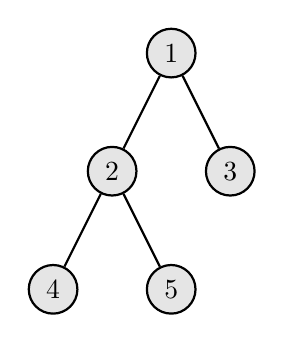
\begin{tikzpicture}
[every node/.style={draw, circle, fill=gray!20!, minimum size=5mm},
thick]
\node{1}
child{node{2} child{node{4}} child{node{5}}}
child{node{3}};
\end{tikzpicture}
\end{figure}
  

\textbf{Output}: \fcj{[[4,5,3],[2],[1]]}
 

\textbf{Explanation}:

Removing the leaves \fcj{[4,5,3]} would result in this tree:

\begin{figure}[H]
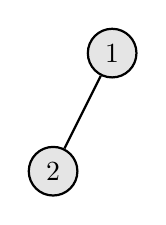
\begin{tikzpicture}
[every node/.style={draw, circle, fill=gray!20!, minimum size=5mm},
thick]
\node{1}
child{node{2}}
child[missing];
\end{tikzpicture}
\end{figure}

Now removing the leaf [2] would result in this tree:

\begin{figure}[H]

\begin{tikzpicture}
[every node/.style={draw, circle, fill=gray!20!, minimum size=5mm},
thick]
\node{1};
\end{tikzpicture}
\end{figure}


Now removing the leaf [1] would result in the empty tree.
\end{flushleft}

\subsection{Find Maximum Height}
We can see the results are sorted by the height of each node, thus we can use the similar recursive approach in finding maximum height

\setcounter{lstlisting}{0}
\begin{lstlisting}[style=customc, caption={DFS}]
vector<vector<int>> findLeaves( TreeNode* root )
{
    vector<vector<int>> ans;
    get_height( root, ans );
    return ans;
}
int get_height( TreeNode* t, vector<vector<int>>& ans )
{
    if( !t )
    {
        return 0;
    }
    //get height of node t
    int h = 1 + ( max )( get_height( t->left, ans ), get_height( t->right, ans ) );
    if( ans.empty() || ( h >= ( int )ans.size() + 1 ) )
    {
        //add another array to hold the values
        ans.emplace_back( vector<int> {} );
    }
    //add t's value to corresponding height
    ans[h - 1].push_back( t->val );
    return h;
}
\end{lstlisting}

